\documentclass{article}




%\let\LaTeXbibliographystyle\bibliographystyle
%\def\bibliographystyle#1{}
\usepackage{arxiv}
\usepackage[superscript,biblabel]{cite}
%\usepackage{ama}
%\let\bibliographystyle\LaTeXbibliographystyle
%\bibliographystyle{ama}

\usepackage[utf8]{inputenc} % allow utf-8 input
\usepackage[T1]{fontenc}    % use 8-bit T1 fonts
\usepackage{hyperref}       % hyperlinks
\usepackage{url}            % simple URL typesetting
\usepackage{booktabs}       % professional-quality tables
\usepackage{amsfonts}       % blackboard math symbols
\usepackage{nicefrac}       % compact symbols for 1/2, etc.
\usepackage{microtype}      % microtypography
\usepackage{lipsum}		% Can be removed after putting your text content
\usepackage{tikz-cd}
\usepackage{caption}

\graphicspath{{./images/}}

\title{Meat \& cancer: a critical review based on causal analysis %\it{(work in progress)}
}

%\date{September 9, 1985}	% Here you can change the date presented in the paper title
%\date{} 					% Or removing it

\author{
%  Any volunteer? \\
%Any Department\\
%  Anywhere\\
  %% examples of more authors
%   \And
 Enrique Otero \\
  Madrid, Spain\\
  %@eoteromuras \\
  \texttt{eoteromuras@gmail.com%\thanks{This paper results from personal research in my leisure time, at the moment not funded by Orange Spain or any other affiliation}
  } \\
  %% \AND
  %% Coauthor \\
  %% Affiliation \\
  %% Address \\
  %% \texttt{email} \\
  %% \And
  %% Coauthor \\
  %% Affiliation \\
  %% Address \\
  %% \texttt{email} \\
  %% \And
  %% Coauthor \\
  %% Affiliation \\
  %% Address \\
  %% \texttt{email} \\
}

\begin{document}
\maketitle

\begin{abstract}
According to World Health Organization (WHO), processed meat has been declared Group 1 carcinogenic to humans. That means that according to epidemiological studies there is a convincing evidence that the agent causes cancer. However, reviewing some of the mainly referred studies with the lenses of causal inference analysis reveals flaws that would invalidate these conclusions. The author(s) intention is to discuss these studies with statistical rigour. By applying last accepted knowledge in the field of causal inference as diagrams and \textit{do-calculus}. With main focus on transparent exposition of health domain assumptions. And the translation of these assumptions into explicit language, diagrams and formulas. So the veracity of domain assumptions can be refuted according to domain expertise. And any conclusion derived from these assumptions being validated or invalidated on the basis of axiomatic logic and maths.

% Despite how unhealthy or unsustainable meat consumption could be, carcinogenic Group 1 statements could be based on uncomplete models, but they at least should be based on correct analysis.
\end{abstract}


% keywords can be removed
\keywords{Meat \and Cancer \and Causality}


\section{Introduction}
 In October 2015 IARC (International Agency for Research on Cancer) held an expert panel that considered the evidence for red and processed meat as possible human carcinogens. They classified processed meat as a Group 1 carcinogenic to humans, and red meat as Group 2A, probably carcinogenic \cite{whoint}. A summary of the final evaluations were published online in The Lancet Oncology \cite{lancet}. And the details of these conclusions were published later in a monograph in 2016 \cite{monograph}.

The consumption of processed meat was associated with small increases in the risk of cancer in the studies reviewed. In these studies, the risk generally increased with the amount of meat consumed \cite{whoint}.


In the next sections we will focus on two studies supporting IARC conclusions, and we will remark different flaws detected in them. Particularly:

\begin{itemize}

\item As starting point, in Section \ref{sec:iarc} we will present IARC monograph and Chan's et al meta-analysis \cite{chan}, as it's the main reference for IARC when they conclude "each 50 gram portion of processed meat eaten daily increases the risk of colorectal cancer by 18\%". We will remark potential problems related to heterogeneity. And some considerations regarding confounders. %Though our focus will be in introducing possible problems related to not conditioning on missing confounders (Section 3), or conditioning on a collider (Section \ref{sec:cross}).
%\item In Section \ref{sec:sandhu} we present Sandhu et al meta-analysis \cite{sandhu} as an example of discarding a plausible confounder based on a possible wrong procedure. Sandhu meta-analysis is both referenced by Chan's \cite{chan} and IARC monograph \cite{monograph}
\item Finally in Section \ref{sec:cross} we'll discuss a study by Cross et al \cite{cross} as an example of generating strange and questionable conclusions based on the wrong procedure of conditioning on a collider. This study is particularly relevant as it's the one that contributes the most to results on Chan's meta-analysis.%\footnote{%Analysis on Section \ref{sec:sandhu} has still much room for improvement. And
%Section \ref{sec:iarc} is maybe unnecessary large. So as an anxious reader you can skip directly to Section \ref{sec:cross}. Anyhow, feedback on the full document would be appreciated, either as a potential collaborator, critical reviewer or helpful hater :) LaTeX source on github \cite{mygithub}}

\end{itemize}

For this purposes we will use different causal inference techniques as causal diagrams and \textit{do-calculus}, as presented by Pearl and Mackenzie \cite{bookofwhy}.

%%%%%%%%%%%
%%%%%%%%%%%
\section{Processed Meat and Colorectal Cancer Incidence}
\label{sec:iarc}

IARC Working Group analysed both "20 large [...] cohort studies [...] extended from as early as the 1990s until the 2010s", and "a large number of case-control studies (approximately 150)".\cite{monograph} The monograph describes also five criteria they applied in reviewing and interpreting the available literature in order to be considered for their meta-analysis. %One of these criteria, which we will focus specifically on this paper is the "Adjustment for potential confounding factors"

Regarding case-control studies, they considered that "approximately 10\% of all case–control studies reviewed were informative for the assessment of the consumption of processed meat in relation to incidence of cancer of the colorectum". Taking into account previous statement of approximately 150 control-studies, they should be 150/10 = 15 informative studies. However they say: "Six of the nine studies considered showed positive associations with cancer of the colorectum." Could this difference (9 vs. 15) be a typo?

In relation to cohort studies, the IARC presented conclusions from a meta-analysis including data from 10
of these studies that "reported a statistically significant dose–response association between consumption
of red meat and/or processed meat and cancer of the colorectum". More concretely, they refer to Chan et al \cite{chan}, where "dose-response relationships were expressed per increment of intake of 100 grams
per day for red and processed meat, and 50 grams per day for processed meat as in previous meta-analyses".\cite{sandhu}%\cite{aicr}


\subsection{Dose-response Analysis on Processed Meat. Heterogeneity and Confounders}

26 publications from 21 studies were included in Chan's meta-analysis \cite{chan}. Being 15 publications from 14 studies on processed meat. Results in Table~\ref{tab:table}.

\begin{table}
 \caption{Summary relative risk of processed meat and colorectal cancer. Chan et al. meta-analysis}
  \centering

  \begin{center}
   \begin{tabular}{||c c c||}
   \hline
   Pooled RR (95\% CI)     & n     & Heterogeneity (I2)\\ [0.5ex]
   \hline\hline
     1.18 (1.10–1.28), P-value=0.00  & 9 & 12\%, P-value=0.33     \\ [1ex]
   \hline
  \end{tabular}

  \caption*{RR – relative risk; CI – confidence interval; n – number of studies}
  \end{center}

  \label{tab:table}
\end{table}

A relatively low I-squared level of 12\% with a relatively high p-value of 0.33 should indicate no significant heterogeneity between studies. So the combined results would not be invalidated. Though criticism has been done to I-squared as an adequate measure of heterogeneity, specially when the number of studies is small. \cite{hippel}.

In relation to confounders, Chan claims: "we cannot rule out residual confounding". Though "in all studies, relative risk estimates were adjusted for age and sex, and all except two adjusted for total energy intake. More than
half of the study results were adjusted for body mass index (BMI), smoking, alcohol consumption, or physical activity, close to half controlled for dairy food or calcium intake, social economic status, family history of colorectal cancer, or plant food or folate intake.
In some studies, the estimates were controlled for use of nonsteroidal anti-inflammatory drugs, fish or white meat intake". %And also: "several potential confounders were not included in the final statistical models in some studies because, as the authors reported, their inclusion in the model did not substantially modified the relative risk estimates." However, sometimes the decision of excluding a confounder could be flawed, not only based on domain assumptions, but also in the logical procedure itself, as we will discuss on the example of Section \ref{sec:sandhu}

Chan's paper refers to other studies with similar conclusions.\cite{aicr,wei2009}
Though it adds also: "In a more recent article on the NHS (Nurses's Health Study) and the HPFS (Health Professionals Follow-up Study), the associations of red meat and processed meat and colon cancer were attenuated after better adjustment for confounders and longer followup".\cite{wei}

The biggest study analysed by Chan's et al\cite{chan} regarding number of people was Cross et al\cite{cross} with 494036 men and women. In this study adjusts were made on "Age, sex, ethnicity, BMI, smoking habits, alcohol intake, physical activity, total energy intake, fruit and vegetable intake, education level, marital status, family history of cancer".
And according to weight and results Cross's study is the one that contributes the most to RR for colorectal cancer on the consumption of processed meat on Chan's meta-analysis. So in section \ref{sec:cross} we'll try to prove that Cross study could be flawed due to implicitly conditioning on a collider.



%\section{Don't Discard Fiber, Vegetables, Fruits or Life-style as Possible Confounders}
%\label{sec:sandhu}
%In 2001 Sandhu et al published a meta-analysis on the relation between meat consumption and colorectal cancer \cite{sandhu}. Discussing about "Meat and Other Dietary and Associated Factors" they wrote: "the current prospective epidemiological data show only a weak negative association between vegetables and fruits consumption and risk of colorectal cancer. Four recent studies, two randomized trials on adenoma recurrence and two large prospective studies [...] found no association among fiber, vegetables, and fruits consumption and risk of colorectal cancer."

%But even if the total effect from fiber, vegetables, and fruits consumption on colorrectal cancer is negligible, matematically the direct effect even could be important. Under the assumption that consumption of vegetables was associated with consumption of meat via dietary lifestyle.

%As an example, considering:

%\begin{itemize}
%\item X: meat
%\item Y: colorrectal cancer
%\item V: vegetables
%\item U: some dietary lifestyle, confounder of V and X
%\end{itemize}

%with the following causal diagram:

%\begin{tikzcd}
%X \arrow{r} &Y\\
%U \arrow{u} \arrow{r} &V \arrow{u}
%\end{tikzcd}

%If "no association among fiber, vegetables, and fruits consumption and risk of colorectal cancer"
%\begin{equation}
%  P(Y|V)=P(Y)
%\end{equation}

%Otherwise, according to the provided causal diagram, V blocks all back-door paths between X and Y. Thus:
%\begin{equation}
%\label{eq:1}
%P(Y|do(X))=\sum _{i=1}^{N} P(Y|X,V_i)P(V_i)
%\end{equation}

%For instance if we consider that V is a binary variable, then:
%\begin{equation}
%\label{eq:1}
%P(Y|do(X))= P(Y|X,\overline V)P(\overline V) + P(Y|X,V)P(V) = P(Y|X)(P(\overline V)+P(V)) = P(Y|X)
%\end{equation}

%On the basis of the previous analysis we still have no evidences that justify to ignore V.

%For instance, in the specific case where X and V are binary variables, U = constant = 1. Thus \begin{equation} X = 1 - V = \overline{V}\end{equation}

%Then:
%\begin{equation}
%P(Y|do(X))=P(Y|X,\overline V)P(\overline V)+P(Y|X,V)P(V) = P(Y|X,X)(1-P(V))+P(Y|X,\overline X)P(\overline X)
%\end{equation}

%So finally:
%\begin{equation}
%P(Y|do(X))=P(Y|X)(1-P(V)) = P(Y|X)\times 1 = P(Y|X)
%\end{equation}


%As an example, ignoring the effect of V we get:

%\begin{tikzcd}
%X \arrow{r} &Y\\
%U \arrow{u} &V
%\end{tikzcd}

%With no backdoor paths between X and Y. So it would be:

%\begin{equation}
%P(Y|do(X))=P(Y|X)
%\end{equation}


%Other of the biggest studies like English et al \cite{english} included also fish as possible cause.

\section{Leukemia versus Life-style Cancers. The Collider Bias}
\label{sec:cross}
As previously said, Cross' analysis, published on 2007 \cite{cross}, was the second biggest study included on Chan's meta-analysis. And the one that partially contributed more to increase the summary relative risk (RRs) for processed meat on colorectal cancer. Chan's pooled estimation of 1.18 was finally included in the IARC monograph \cite{monograph} and into WHO's claim \cite{whoint}. But ignoring Cross' study could reduce Chan's pooled RR from 1.18 to 1.10.

In this context, we will show in this section an example of probable bad control in Cross' study leading to some strange results.

Extracted from Cross' analysis: "Surprisingly, both leukemia and melanoma were inversely associated with processed meat intake; the inverse association for leukemia was mainly for lymphocytic leukemia (n = 534; HR\footnote{HR stands for Hazard Ratio.
%, not related to the brand new unworn Real Madrid player. Joking aside,
It would be also interesting to go deeper into how Cross's Hazard Ratios (HR) have been converted to Chan's pooled Relative Risks (RR). Being these metrics similar but not the same} = 0.70; 95\% CI = 0.52–0.93; p for trend = 0.05) and not myeloid and monocytic leukemia (n = 457; HR = 0.88; 95\% CI = 0.64–1.20; p for trend = 0.73)."\cite{cross}

But according to described cohort follow-up: "[it] was calculated from baseline (1995–1996) until censoring at the end of 2003, or when the participant moved out of one of the eight study areas, had a cancer diagnosis, or died, whichever came first" \cite{cross}. Thus, analysing several types of cancer as target while implicitely conditioning on not having any other cancer converts the variable "any cancer" in a collider.

Considering
\begin{itemize}
\item X: processed meat
\item Y: leukemia
\item C1: colorectal cancer
\item C: any type of cancer
\end{itemize}

and assuming the following causal diagram:

\begin{tikzcd}
X \arrow{d} \arrow{r} &Y \arrow{d}\\
C1 \arrow{r} &C
\end{tikzcd}

So conditioning on the collider C opens the path Y -> C <- C1 <-X, invalidating the results of the study. This situation is typically known as \textit{collider bias}. Being a well known example the \textit{Berkson Paradox} described for instance in Pearl and Mackenzie's \textit{The Book of Why}.\cite{bookofwhy}

And this could explain these strange results, where cancers as colorectal, usually associated with dietary lifestyle, have Hazard Ratios above 1 (HR=1.2), whereas leukemia shows apparently an inverse relation to processed meat, with an HR of 0.7. As we can see in Figure \ref{fig:cross}.
\begin{figure}
  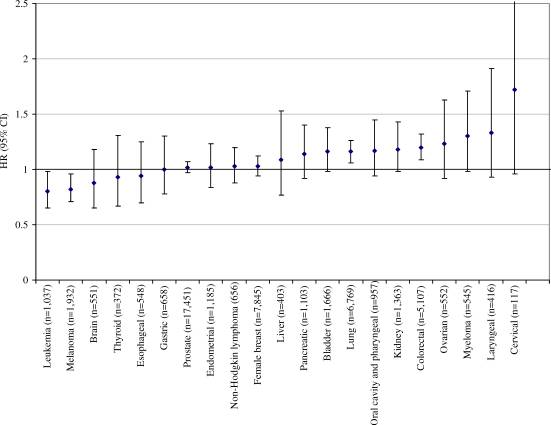
\includegraphics[scale=0.75]{tileshop2}
  \caption{HRs and 95\% CIs for the 5th Versus 1st Quintile of Processed Meat Intake and Cancer Risk for Both Sexes Combined (Except for Sex-Specific Cancers). From Cross et al.\cite{cross}}
  \label{fig:cross}
\end{figure}


%Furthermore, this study includes some other strange conclusions, some of them also due to the collider bias, some apparently not. For instance: "we observed a suggestion of an elevated risk for advanced prostate cancer (n = 1,782), for both red meat (HR = 1.15; 95\% CI = 0.98–1.36; p for trend = 0.21) and processed meat intake (HR = 1.22; 95\% CI = 1.05–1.43; p for trend = 0.08), when comparing those in the highest with those in the lowest quintile of intake". Seems a little surprising, taking into account Figure \ref{fig:cross}, and the detailed values given for prostate cancer showing HR=1.01 (0.97-1.06) for the lowest and HR=1.02 (0.97-1.07) for the highest quintile. Cross et al finally conclude that "the relation of meat intake to prostate cancer is confined to advanced disease"

Moreover even despite or because of the collider bias some patterns could be noticed. For instance, between the 4 most prevalent types of cancer, colorectal and lung cancer show similar results in this study, with higher HR values. While prostate and female breast show values closer to 1. Besides, Cross et al point that "a stepwise addition of the covariates to a simple age- and sex-adjusted model showed that the effects of red and processed meat intake on cancer risk were attenuated the most by the addition of the smoking variable to the models". %smoking-meat paradox? smells like collider or counfounder spirit.

All this patterns and hints could be useless because of the collider bias. Or they could indicate "dietary" and/or "life style" as possible confounder of both meat consumption and smoking and some types of cancers as colorectal or lung. While prostate or breast cancer would be less dependent from presumptive or proved bad habits. %\footnote{It would be great if we could demonstrate someday this hypothesis of "dietary" \& "life-style" cancers. Or at least trying to do it}


\section{Conclusions}

%\textbf{\textit{To be finished...}}
Processed meat has been classified by WHO as Group 1 carcinogenic to humans \cite{whoint}. Several analysis have been considered to generate this conclusion. Specifically, WHO claims that "an analysis of data from 10 studies estimated that every 50 gram portion of processed meat eaten daily increases the risk of colorectal cancer by about 18\%". This conclusion comes from Chan's et al meta-analysis \cite{chan}. And this meta-analysis has been highly dependent on Cross's et al study \cite{cross}.

First of all some criticism could be made on the heterogeneity of Chan's meta-analysis. And I-squared as an inadequate measure of this heterogeneity in this case due to the small number of studies \cite{hippel}.

But our goal was to review with "causal glasses" the association between meat and cancer. And our main contribution was to demonstrate that Cross's case study is an example of collider bias. Calling into question Chan's conclusions and WHO's claim.

Moreover, explicitly showing assumptions and causal diagrams can help synergies between health domain and causal inference in statistics. Avoiding knowledge silos and contributing to new advances on nutrition and cancer research.


\section{Funding}
The author(s) received no financial support for the research, authorship, and/or publication of this article.

\bibliographystyle{unsrt}
%\bibliography{references}  %%% Remove comment to use the external .bib file (using bibtex).
%%% and comment out the ``thebibliography'' section.


%%% Comment out this section when you \bibliography{references} is enabled.
\begin{thebibliography}{1}

\bibitem{whoint}
Q\&A on the carcinogenicity of the consumption of red meat and processed meat. World Health Organization. https://www.who.int/features/qa/cancer-red-meat/en/. Published October 2015. Accessed September 3, 2019.

\bibitem{lancet}
Bouvard V, Loomis D, Guyton K et al. Carcinogenicity of consumption of red and processed meat. Lancet Oncol. 2015;16(16):1599-6006
%\newblock https://www.researchgate.net/profile/Veronique\_Bouvard/publication/283443910\_Carcinogenicity\_of\_consumption\_of\_red\_and\_processed\_meat/links/5ac393f4aca272a2c99910f1/Carcinogenicity-of-consumption-of-red-and-processed-meat.pdf

\bibitem{monograph}
IARC Monographs on the Evaluation of Carcinogenic Risks to Humans. Red Meat and Processed Meat. Vol 114. International Agency for Research on Cancer. https://monographs.iarc.fr/wp-content/uploads/2018/06/mono114.pdf. Published June 2018. Accessed September 3, 2019.

\bibitem{chan}
Chan D, Lau R, Aune D et al. Red and Processed Meat and Colorectal Cancer Incidence: Meta-Analysis of Prospective Studies. PLoS One. 2011;6(6):e20456
%https://journals.plos.org/plosone/article/file?id=10.1371/journal.pone.0020456\&type=printable

\bibitem{cross}
Cross AJ, Leitzmann MF, Gail MH, Hollenbeck AR, Schatzkin A, Sinha R. A prospective study of red and processed meat intake in relation to cancer risk. PLoS Med. 2007;4(12):e325. doi:10.1371/journal.pmed.0040325

\bibitem{bookofwhy}
Pearl J, Mackenzie D. The Book of Why. The New Science of Cause and Effect. New York, NY: Basic Books; 2018.

\bibitem{sandhu}
Sandhu MS, White IR, McPherson K. Systematic review of the prospective cohort studies on meat consumption and colorectal cancer risk: a meta-analytical approach. Cancer Epidemiol Biomarkers Prev. 2001 May;10(5):439-46.

\bibitem{hippel}
Von Hippel PT. The heterogeneity statistic I2 can be biased in small meta-analyses. BMC Med Res Methodol. 2015 Apr 14;15:35. doi: 10.1186/s12874-015-0024-z.

\bibitem{aicr}
World Cancer Research Fund / American Institute for Cancer Research.
Food, Nutrition, Physical Activity, and the Prevention of Cancer: a Global
Perspective. Washington, DC: American Institute for Cancer Research. https://www.wcrf.org/sites/default/files/english.pdf. Published 2007. Accessed September 3,2019.

\bibitem{wei2009}
Wei EK, Colditz GA, Giovannucci EL, Fuchs CS, Rosner BA. Cumulative risk of colon cancer up to age 70 years by risk factor status using data from the Nurses’ Health Study. Am J Epidemiol. 2009 Oct 1;170(7):863-72. doi: 10.1093/aje/kwp210.

\bibitem{wei}
Wei EK, Giovannucci E, Wu K et al. Comparison of risk factors for colon and rectal cancer. Int J Cancer. 2004 Jan 20;108(3):433-42.2.

%\bibitem{english}
%English DR, MacInnis RJ, Hodge AM, Hopper JL, Haydon AM, et al. (2004)
%Red meat, chicken, and fish consumption and risk of colorectal cancer. Cancer
%Epidemiol Biomarkers Prev 13: 1509–1514.



%\bibitem{mygithub}
%LaTeX source for this draft paper:
%https://github.com/muoten/arxiv-style/blob/master/meat\_and\_cancer.tex
\end{thebibliography}



\end{document}
